\documentclass{beamer}
\usepackage[utf8]{inputenc} % allow utf-8 input
\usepackage[T1]{fontenc}    % use 8-bit T1 fonts
\usepackage{url}            % simple URL typesetting
\usepackage{booktabs}       % professional-quality tables
\usepackage{amsmath,amsthm,amsfonts,amssymb}       % blackboard math symbols
\usepackage{nicefrac}       % compact symbols for 1/2, etc.
\usepackage{microtype}      % microtypography
\usepackage{xcolor}         % colors
\usepackage{graphicx}
\usepackage{float}
\usepackage{algpseudocode}
\usepackage{algorithm}
% \usepackage[capitalise]{cleveref}
\usepackage{hyperref}
\usepackage{caption, subcaption}
\usepackage{adjustbox}
\usepackage{multimedia}
\algnewcommand\algorithmicforeach{\textbf{for each}}
\algdef{S}[FOR]{ForEach}[1]{\algorithmicforeach\ #1\ \algorithmicdo}

\newcommand{\e}[1]{\mathbb{E}(#1)}
\setbeamercovered{transparent}
\setbeamertemplate{itemize items}[triangle]
% \setbeamertemplate{footline}[frame number]
\title{Q Learning and Deep Q Network}
\author{Ling Fei Zhang\\
    260985358}

\usetheme{Darmstadt}
\usecolortheme{seahorse}
% \setbeamertemplate{section in toc}[circle]

\begin{document}
\maketitle

\begin{frame}
    \frametitle{Table of Contents}
    \tableofcontents
\end{frame}

\section{Introduction}

\begin{frame}
    \frametitle{Games}
    \begin{columns}
        \column{0.5\textwidth}
        \centering
        CartPole
        \medskip
        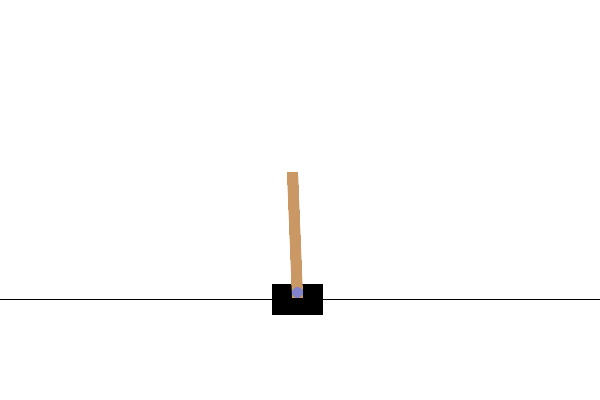
\includegraphics[width=\textwidth]{cart_pole.png}
        \column{0.5\textwidth}
        \centering
        Lunar Lander
        \medskip
        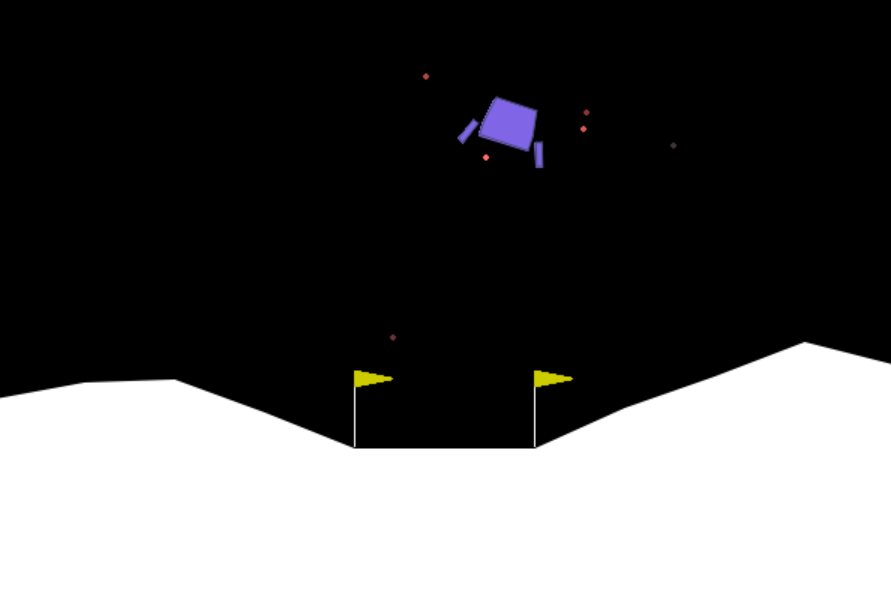
\includegraphics[width=\textwidth]{lunar.png}
    \end{columns}
\end{frame}

\begin{frame}
    \frametitle{Agents}
    \begin{itemize}
        \item Q Learning \pause
              \begin{itemize}
                  \item Model-free reinforcement learning algorithm \pause
                  \item Uses a table to store Q values for each state-action pair \pause
                  \item Effective in simple environments\pause
                  \item Struggles in more complexe environments since it is impractical to store and
                        update Q values for all the state-action pairs\pause
              \end{itemize}
        \item Deep Q Network (DQN) \pause
              \begin{itemize}
                  \item Uses neural networks to learn policies to map states to Q values\pause
                  \item Neural networks can handle large state spaces and continuous action spaces
              \end{itemize}
    \end{itemize}
\end{frame}

\section{Background}
\begin{frame}
    \frametitle{Background}
    \begin{itemize}
        \item Future discounted return at time \(t: R_t =
              \sum_{t'=t}^{T}\gamma^{t'-t}r_{t'}\) \pause
        \item The optimal action-value function \(Q^*(s,a) = \max_\pi \e{R_t | s_t = s, a_t =
                  a, \pi}\) \pause
        \item Optimal stragery is to maximize the expected value of \(r + \gamma Q^*(s',a')\)
    \end{itemize}

\end{frame}

\section{Methodology}

\begin{frame}
    \frametitle{Q Learning Algorithm}

    \begin{algorithm}[H]
        \caption{Q Learning(episodes, \(\alpha, \epsilon, \gamma\))}
        \label{alg:qlearning}
        \begin{algorithmic}[1]
            \State Initialize \(Q(s,a)\) for all \(s \in \mathcal{S}, a \in \mathcal{A}(s)\) arbitrarily
            \State Set \(Q(terminal, \cdot) = 0 \) for all terminal states
            \ForEach {episode in episodes}
            \State Initialize \(s\)
            \State \(done\) \(\leftarrow\) False
            \While {not \(done\)}
            \State Choose \(a \in \mathcal{A}\) from \(s\) using policy derived from \(Q\)
            \State Take action \(a\) and observe reward \(r\) and next state \(s'\)
            \State \(Q(s, a) \leftarrow Q(s, a) + \alpha \left[r + \gamma \max_{a} Q(s', a) - Q(s, a)\right]\)
            \State \(s \leftarrow s'\)
            \EndWhile
            \EndFor
        \end{algorithmic}
    \end{algorithm}

\end{frame}

\begin{frame}
    \frametitle{Q Learning}

    \begin{itemize}
        \item Q Learning uses a table to store Q values for each state-action pair \pause
        \item Impractical to store all Q values for a continuous observation space \pause
        \item Discretization needed \pause
        \item Hyperparameters used for Q Learning\pause
              \begin{itemize}
                  \item Discount factor \(\gamma = 0.99\)
                  \item Start epsilon of 1
                  \item End epsilon of 0.001
                  \item Epsilon decay of \(5^{-4}\)
                  \item 10 bins
                  \item learning rate of 0.25 and 0.005 for CartPole and Lunar Lander, respectively
              \end{itemize}
    \end{itemize}

\end{frame}

\begin{frame}
    \frametitle{DNQ Algorithm Setup}

    \begin{itemize}
        \item Implementation of \texttt{ReplayMemory}, which acts as a replay buffer \pause
        \item Implementation of deep neural network \pause
              \begin{itemize}
                  \item Two hidden layers, each with 128 units
                  \item ReLU activation function
                  \item Adam's optimizer
                  \item Huber loss
              \end{itemize}
    \end{itemize}

\end{frame}

\begin{frame}[shrink=38]
    \frametitle{DQN Algorithm}
    \begin{columns}
        \column{0.7\textwidth}
        \begin{algorithm}[H]
            \caption{DQN(episodes, \(\alpha, \epsilon, \gamma, C\))}
            \label{alg:dqn}
            \begin{algorithmic}[1]
                \State Initialize replay buffer \(\mathcal{D}\) with maximum capacity 100000
                \State Initialize policy network \(Q\) with random weights \(\theta\)
                \State Initialize target network \(\tilde{Q}\) with random weights \(\tilde{\theta}\)
                \ForEach{episode in episodes}
                \State Initialize \(s\)
                \State Set \(t \leftarrow 0\)
                \State \(done\) \(\leftarrow\) False
                \While {not \(done\)}
                \State Choose \(a \in \mathcal{A}\) from \(s\) using policy network \(Q\)
                \State Take action \(a\) and observe reward \(r\), next state \(s'\) and \(done\)
                \State Store transition \((s, a, r, s', done)\)
                \State Sample a minibatch of random transitions \((s, a, r, s', done)\) from \(\mathcal{D}\)
                \State Set \(\hat{y} =
                \begin{cases}
                    r                                                  & \quad \text{if }s \text{ is a terminal state} \\
                    r + \gamma \max_a \tilde{Q}(s', a; \tilde{\theta}) & \quad \text{otherwise}
                \end{cases}\)
                \State Perform gradient descent on \(\left(\hat{y} - Q(s, a; \theta)\right)^2\) w.r.t. the policy network parameters \(\theta\)
                \If {\(t \text{ mod } C = 0\)}
                \State \(\tilde{Q} \leftarrow Q\)
                \EndIf
                \EndWhile
                \EndFor
            \end{algorithmic}
        \end{algorithm} \pause
        \column{0.3\textwidth}
        \begin{itemize}
            \item Discount factor \(\gamma = 0.99\)
            \item Learning rate 0.003
            \item Start epsilon of 1
            \item End epsilon of 0.01
            \item Epsilon decay of \(5^{-4}\)
            \item \(\tau = 0.005\)
            \item Default batch size of 64
        \end{itemize}
    \end{columns}

\end{frame}

\section{Results}

\begin{frame}
    \frametitle{Plots}
    \begin{figure}
        \centering
        \begin{subfigure}[H]{0.49\textwidth}
            \centering
            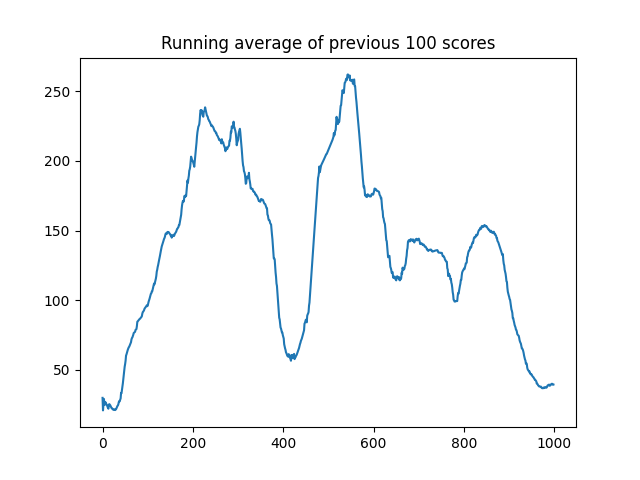
\includegraphics[width=\textwidth]{../plots/cartpole}
            \caption{CartPole}
            \label{fig:cartpole}
        \end{subfigure}
        \begin{subfigure}[H]{0.49\textwidth}
            \centering
            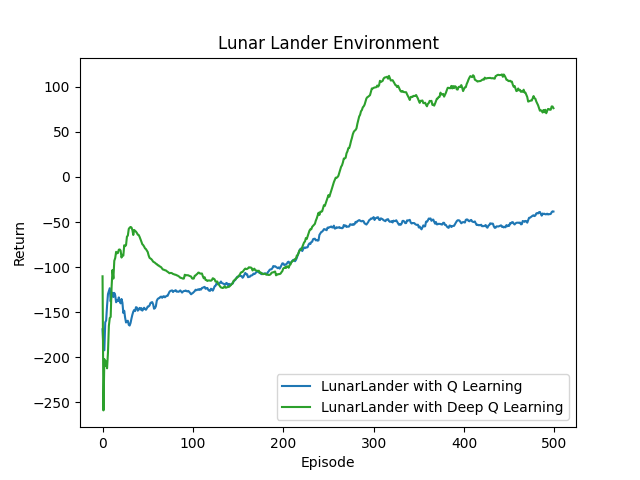
\includegraphics[width=\textwidth]{../plots/lunar}
            \caption{Lunar Lander}
            \label{fig:lunar}
        \end{subfigure}
        \caption{500 training episodes for Q Learning and DQN. Returns are averaged over the last 100 episodes.}
        \label{fig:train}
    \end{figure}

\end{frame}

\begin{frame}
    \frametitle{CartPole}
    DQN\pause
    \begin{itemize}
        \item Learns much quicker than Q Learning \pause
        \item Reached an average return of 300 at around 300 episodes \pause
        \item Unstable learning process: significant drop at episode 350 \pause
        \item Agent is possibly trying to escape a local minimum \pause
    \end{itemize}
    Q Learning\pause
    \begin{itemize}
        \item Learns much slower compared to DQN \pause
        \item Not great returns, even after 500 training episodes \pause
        \item Agent might be stuck in a local minima
    \end{itemize}

\end{frame}

\begin{frame}
    \frametitle{Lunar Lander}

    DQN \pause
    \begin{itemize}
        \item DQN outperforms Q Learning \pause
        \item Unstable learning process \pause
    \end{itemize}
    Q Learning \pause
    \begin{itemize}
        \item Slow but stable learning \pause
        \item No drastic change in average return. Instead, the average return slowly
              increases
    \end{itemize}

\end{frame}

\section{Conclusion}

\begin{frame}
    \frametitle{Conclusion}

    DQN \pause
    \begin{itemize}
        \item Learns much faster in both games, but the agent exhibited some instability
              during the learning process \pause
    \end{itemize}
    Q Learning \pause
    \begin{itemize}
        \item Learns much slower, but more steadily \pause
    \end{itemize}
    \medskip
    \textbf{The choice of algorithm depends on the specific application and trade-offs between speed and stability.}

\end{frame}

\begin{frame}
    \frametitle{Future Work}

    Deep deterministic policy gradient (DDPG) \pause
    \begin{itemize}
        \item Combines Q Learning with policy gradients to learn a deterministic policy
              directly \pause
        \item This has shown to be effective in continuous action spaces and could address
              some of the instability issues observed in DQN.
    \end{itemize}

\end{frame}

\end{document}